
\chapter{Network}

\section{Share your network through wifi}
\label{sec:share-your-network-through-wifi}

As your computer are connecting to Internet thought USB cable line,
you can share you network though wifi to save your phone's packets.
The procedures are as follows:
\begin{itemize}
\item Open ``System Preferences'' (Figure \ref{fig:system-perferences})
  \begin{figure}[!ht]
    \centering
    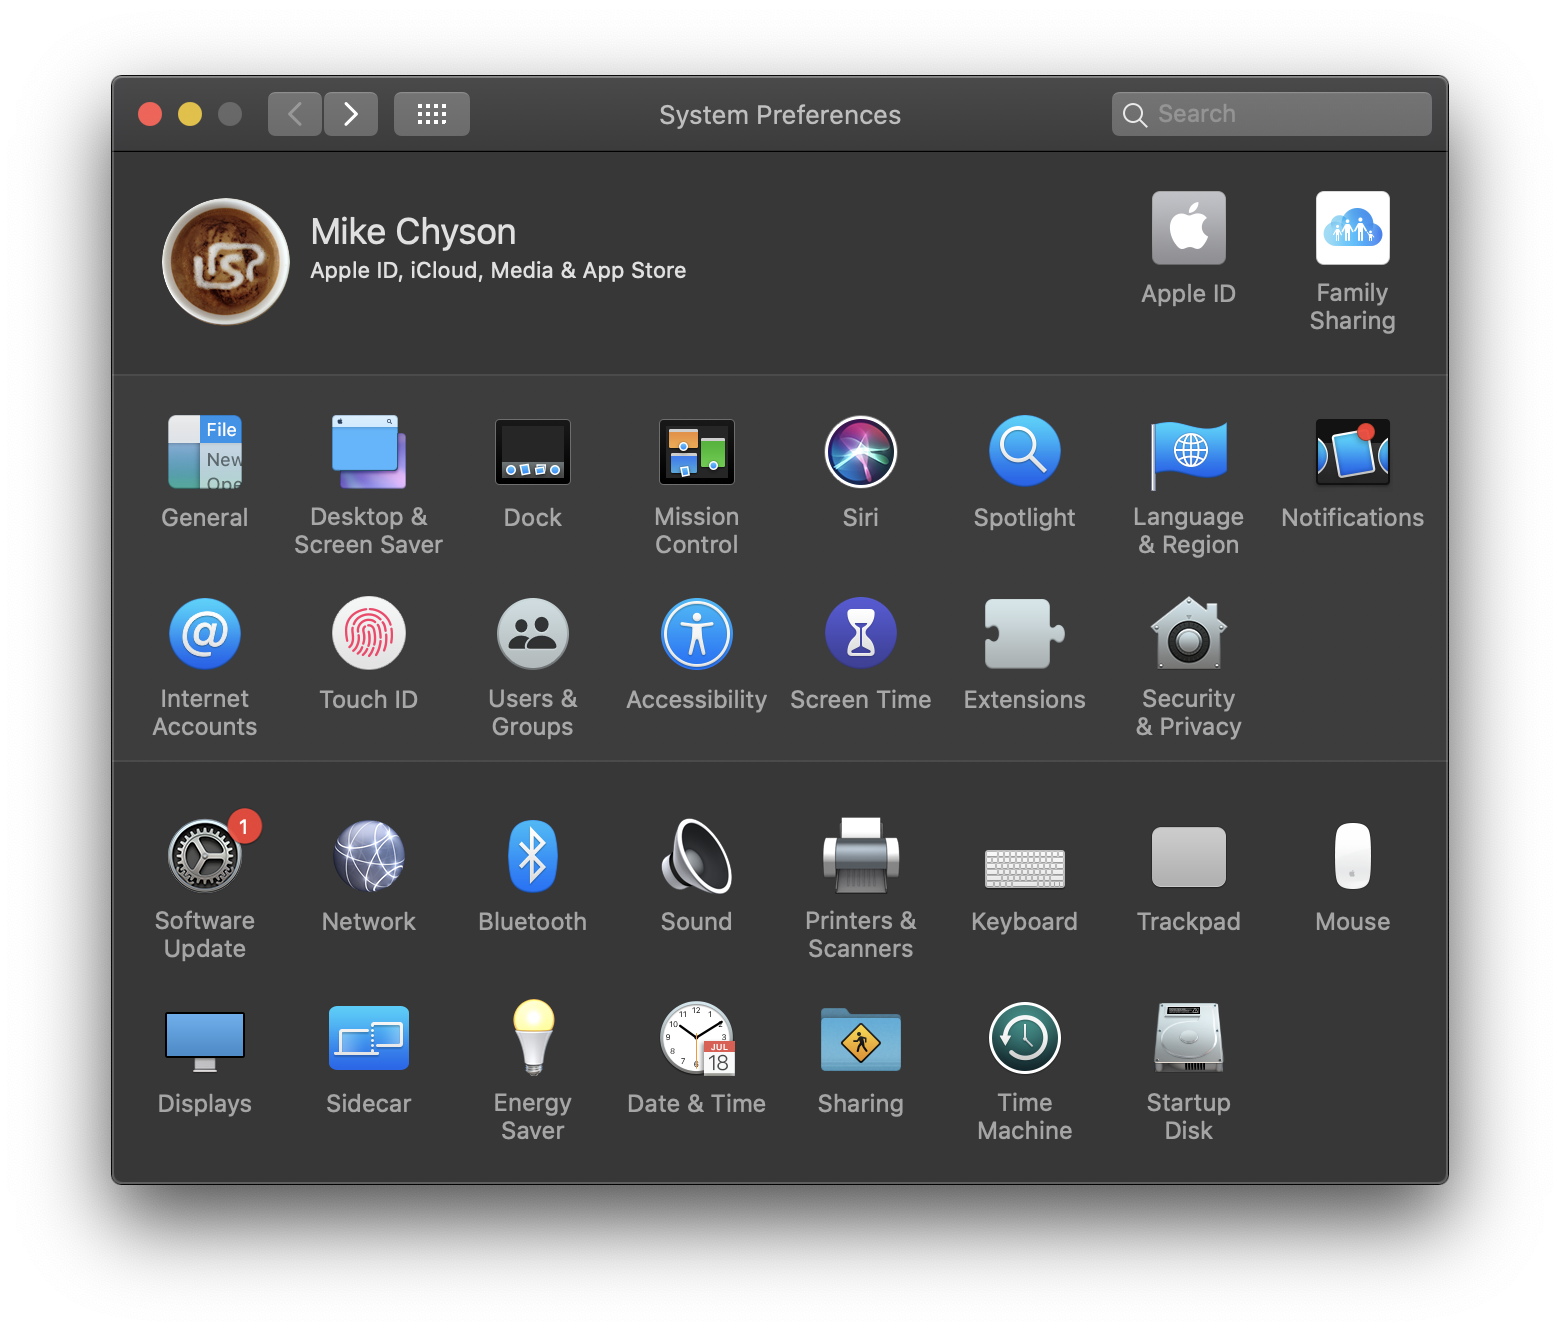
\includegraphics[width=\textwidth]{pics/system-preferences.png}
    \caption{System preferences}
    \label{fig:system-perferences}
  \end{figure}
\item Enter ``Sharing'' (Figure \ref{fig:sharing})
  \begin{figure}[!hb]
    \centering
    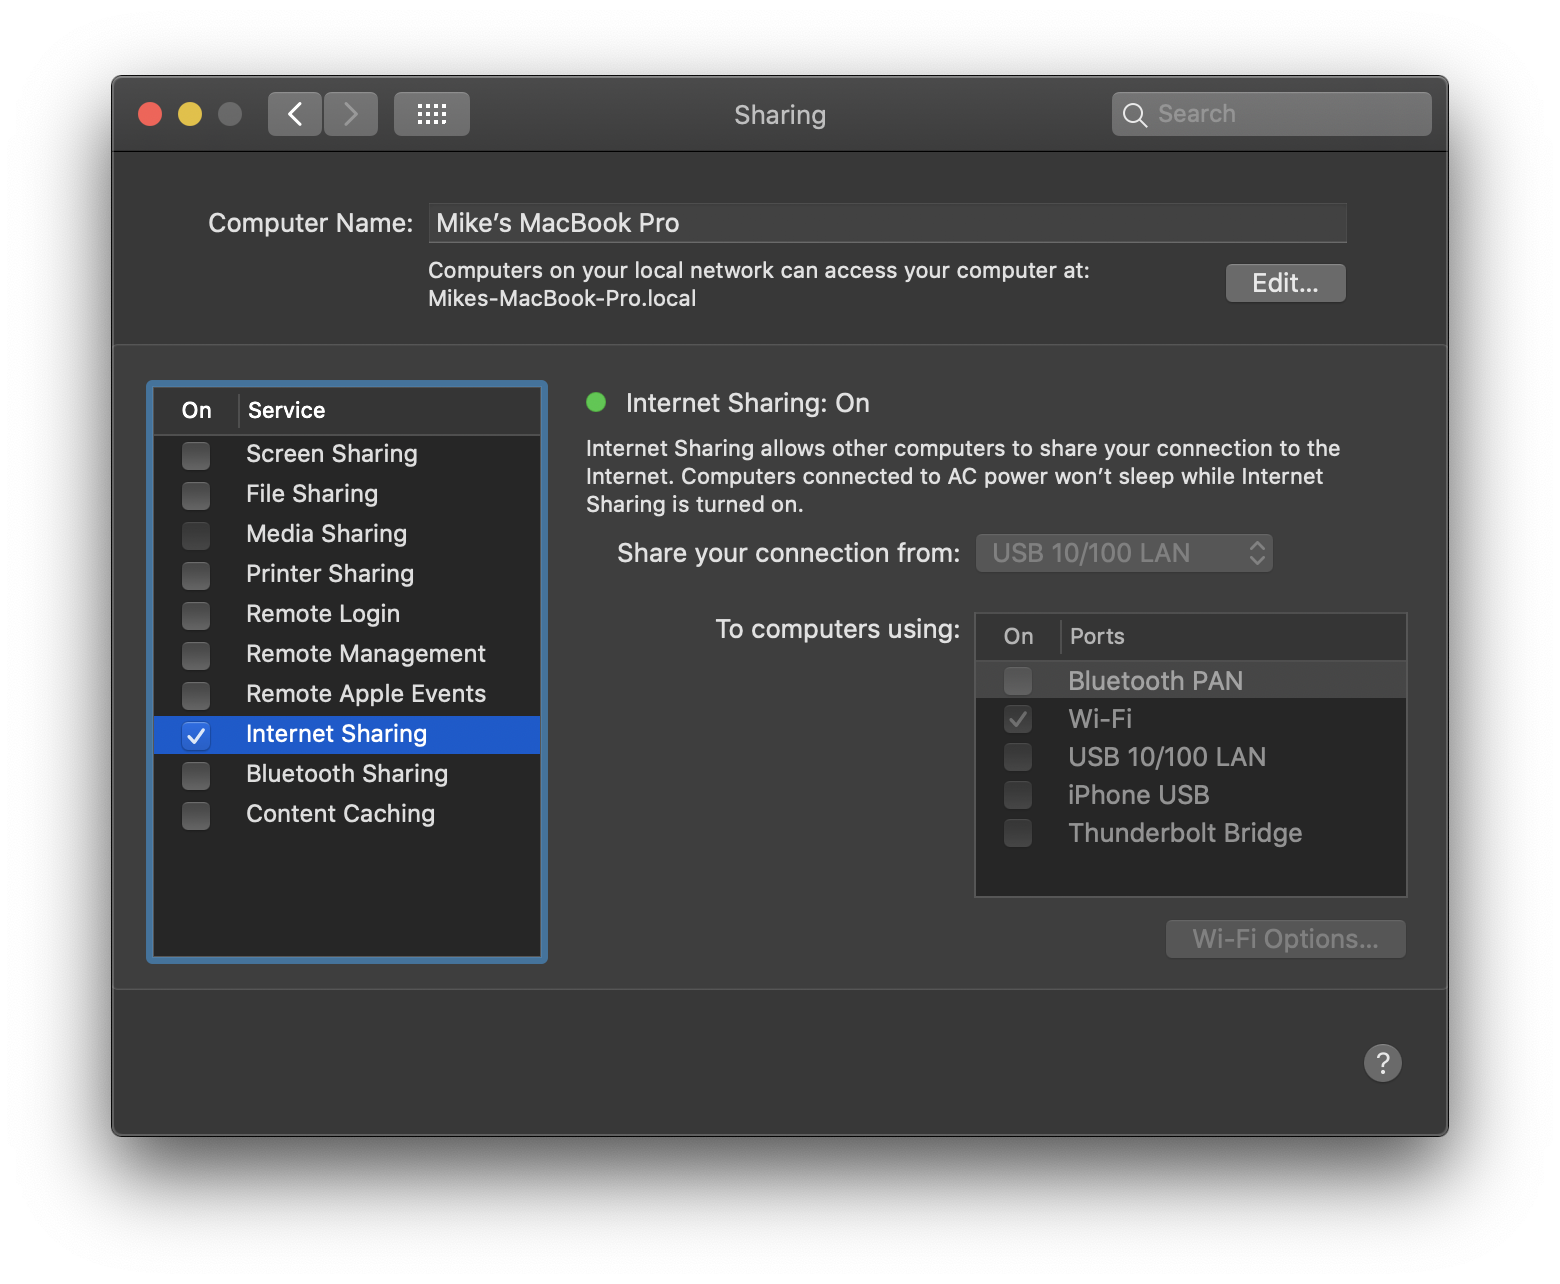
\includegraphics[width=\textwidth]{pics/sharing.png}
    \caption{Sharing}
    \label{fig:sharing}
  \end{figure}
\item The configuration is as shown in Figure \ref{fig:sharing}.
\item To change password, enter the ``Wi-Fi Options''.
\end{itemize}


\section{Share your network through eth}

The configuration is similar to \ref{sec:share-your-network-through-wifi}.

Before you share your network, there is one more thing to do as shown in Figure \ref{fig:computer-to-computer}:
\begin{figure}[!ht]
  \centering
  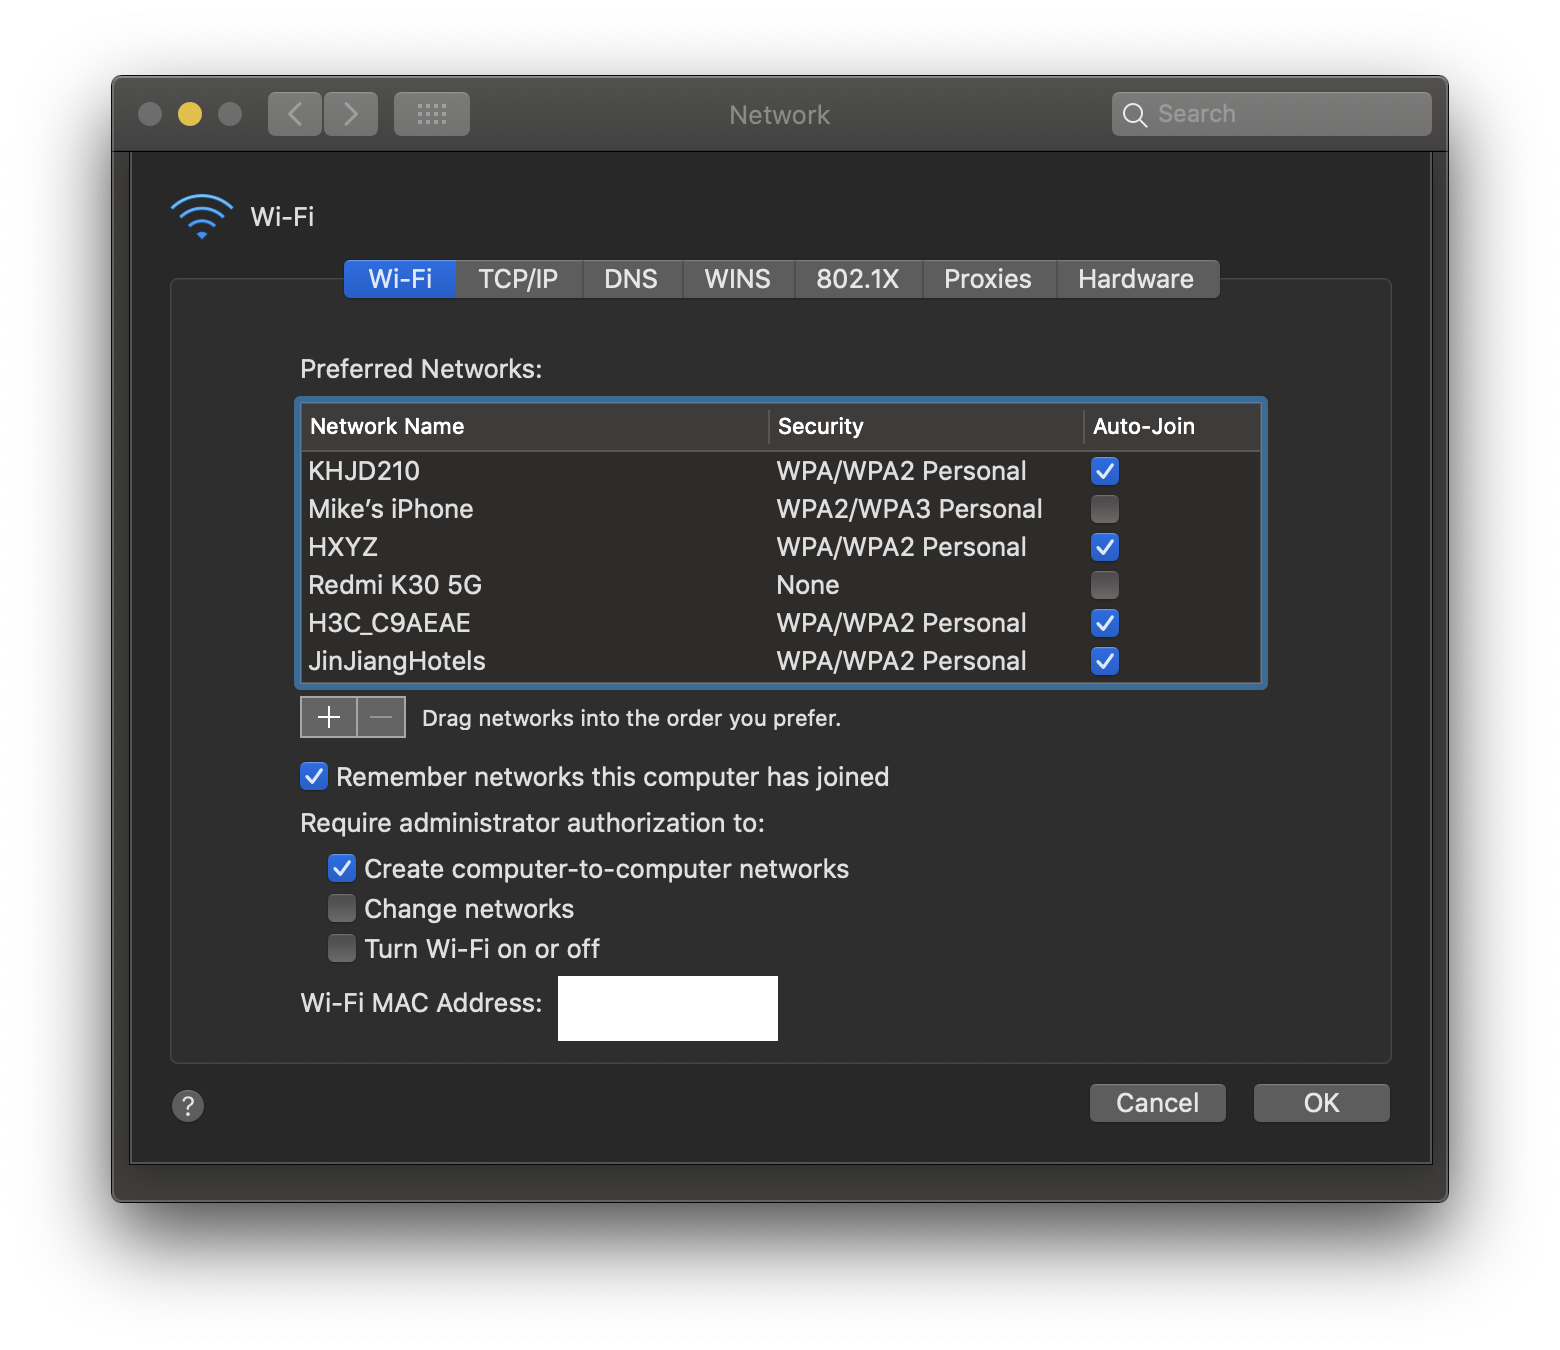
\includegraphics[width=\textwidth]{pics/computer-to-computer.png}
  \caption{Computer to computer network}
  \label{fig:computer-to-computer}
\end{figure}

The sharing configuration is shown in Figure \ref{fig:share-through-eth}
\begin{figure}[!ht]
  \centering
  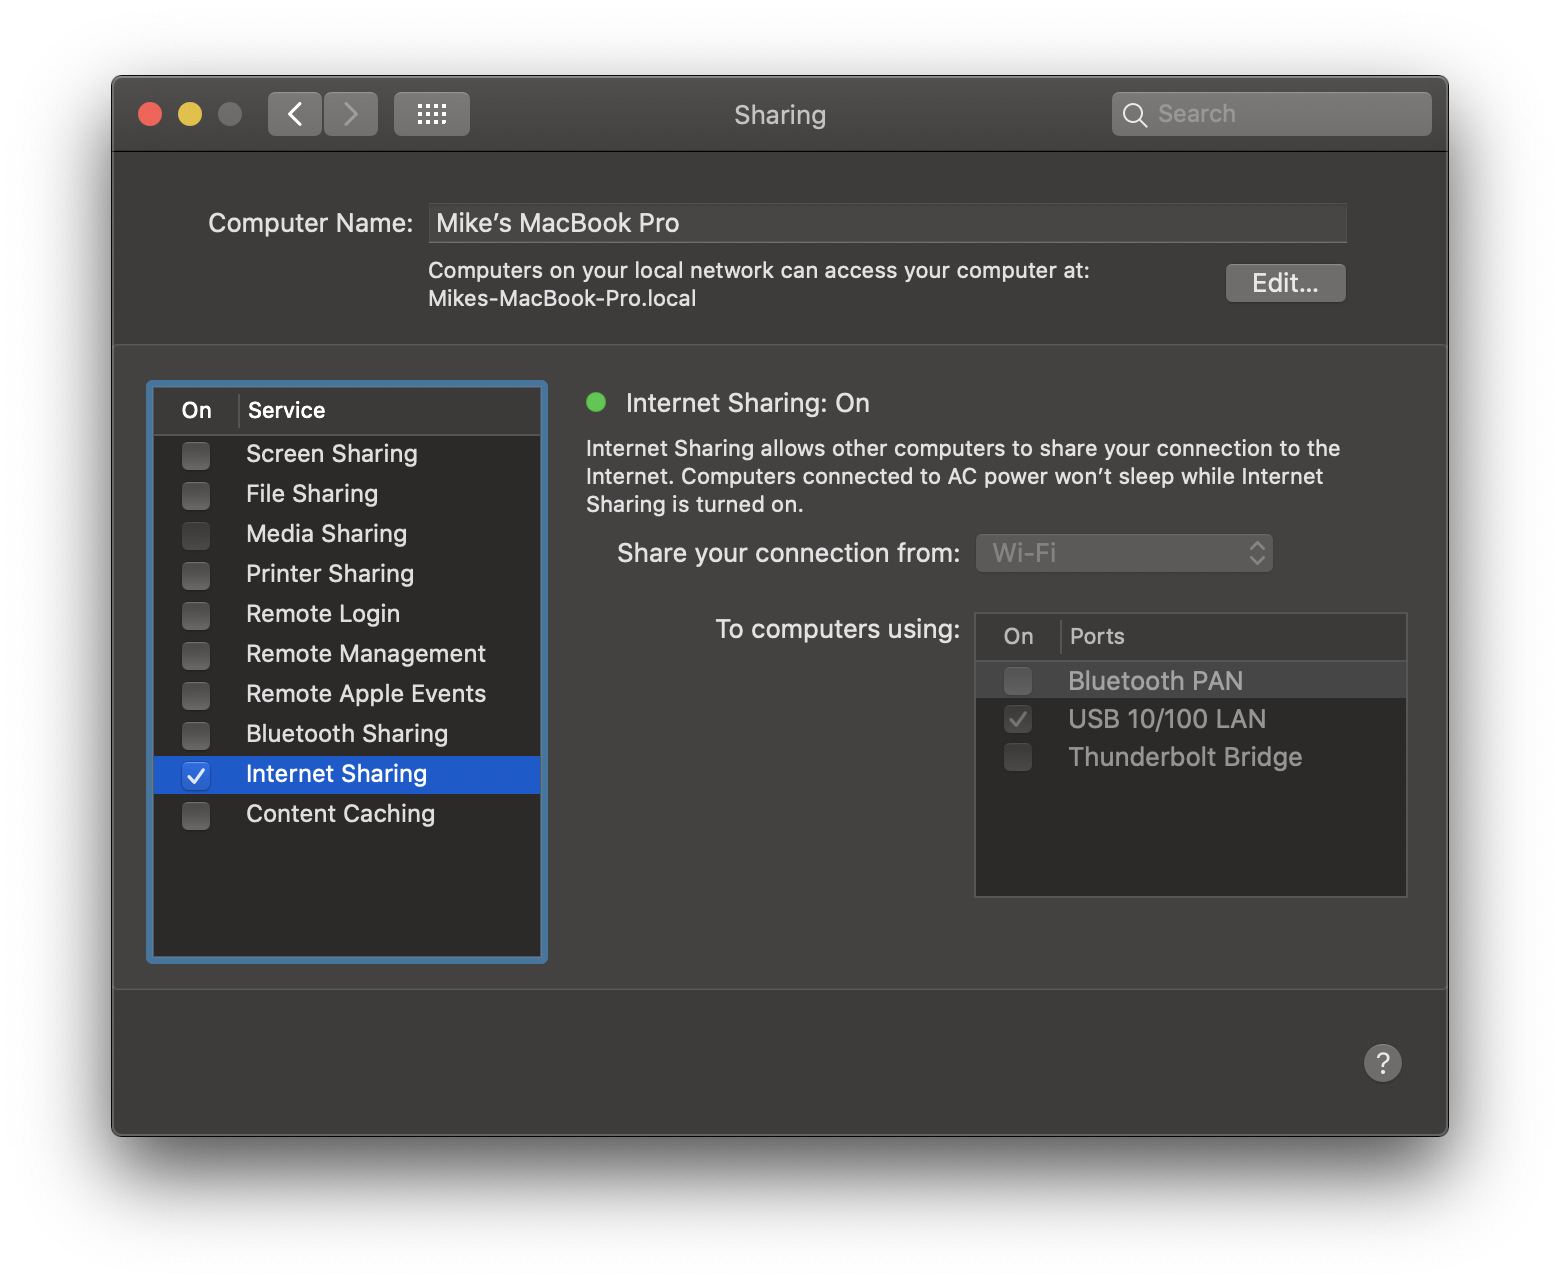
\includegraphics[width=\textwidth]{pics/share-through-eth}
  \caption{Share network through eth}
  \label{fig:share-through-eth}
\end{figure}



\section{Get an American apple id}

\subsection{Phone}

The hard point is to get an Amercian phone nunmber.
Here I use anttone.